\input{styleDS}
\usepackage{enumitem}
\def\numero{Révisions 1}
\def\classe{Option info MP1}
\renewcommand*{\arraystretch}{1.2}
\usetikzlibrary[automata]

\camltrue
%-------------------------------------------------------------------------------
%-------------------------------------------------------------------------------
%-------------------------------------------------------------------------------
\begin{document}
%-------------------------------------------------------------------------------
%-------------------------------------------------------------------------------
%-------------------------------------------------------------------------------
\chapter{Morphismes d'automates, Mines 2019}
%-------------------------------------------------------------------------------
%-------------------------------------------------------------------------------
%-------------------------------------------------------------------------------
{\bf Remarque} : on peut regretter que les composantes de l'automate soient sous forme d'un tuple plutôt qu'un enregistrement.
%-------------------------------------------------------------------------------
%-------------------------------------------------------------------------------
%-------------------------------------------------------------------------------
\section{Premiers exemples}
%-------------------------------------------------------------------------------
%-------------------------------------------------------------------------------
%-------------------------------------------------------------------------------
\begin{Exercise}
${\cal A}_1$ reconnaît les mots de longueur impaire.
\end{Exercise}
%-------------------------------------------------------------------------------
%-------------------------------------------------------------------------------
\begin{Exercise}
${\cal A}_2$ reconnaît les mots qui contiennent un nombre impair de $b$.
\end{Exercise}
%-------------------------------------------------------------------------------
%-------------------------------------------------------------------------------
\begin{Exercise}
Le langage reconnu par ${\cal A}_1$ peut être dénoté par \type{(a+b).(a.a+a.b+b.a+b.b)*}.

On a éliminé quelques parenthèses.
\end{Exercise}
%-------------------------------------------------------------------------------
%-------------------------------------------------------------------------------
\begin{Exercise}
Le langage reconnu par ${\cal A}_2$ peut être dénoté par \type{a*.b.(a + b.a*.b)*}.
\end{Exercise}
%-------------------------------------------------------------------------------
%-------------------------------------------------------------------------------
\begin{Exercise}
\begin{lstlisting}
let q = (2, [|(0, 1); (1, 0)|], [|false; true|]|];; 
\end{lstlisting}
\end{Exercise}
%-------------------------------------------------------------------------------
%-------------------------------------------------------------------------------
%-------------------------------------------------------------------------------
\section{États accessibles}
%-------------------------------------------------------------------------------
%-------------------------------------------------------------------------------
%-------------------------------------------------------------------------------
\begin{Exercise}
Plutôt qu'une convention $-1$ pour un élément non présent, un type optionnel (\type{Some k/None}) aurait été préférable.

\begin{lstlisting}
let numero k liste = 
  let reponse  = Array.make k (-1) in
  let rec aux reste pos =
    match reste  with
    |[] -> reponse
    |t::q -> reponse.(t) <- pos; 
             aux q (pos +1) in
  aux liste 0;;
\end{lstlisting}
La fonction indique la dernière position de l'élément dans la liste.
\end{Exercise}
%-------------------------------------------------------------------------------
%-------------------------------------------------------------------------------
\begin{Exercise}
Comme la question l'indique on parcourt le graphe en profondeur, la formulation récursive est la plus simple.

On accumule les sommets parcourus dans une liste (référencée), l'ordre sera inversé donc on retourne la liste à la fin.
\begin{lstlisting}
let etats_accessibles q =
  let n, delta, f = q in
  let vus = Array.make n false in
  let sommets = ref [] in
  let rec aux s = 
    if not vus.(s)
    then begin
           vus.(s) <- true;
           sommets := s :: !sommets;
           let succ_a, succ_b = delta.(s) in
           aux succ_a;
           aux succ_b end in
  aux 0;
  List.rev !sommets;;   
\end{lstlisting}
\end{Exercise}
%-------------------------------------------------------------------------------
%-------------------------------------------------------------------------------
\begin{Exercise}
On part de la liste des sommets accessibles et on construit un nouvel automate dont les états sont ceux de la liste, ils sont donc numérotés par leur position dans la liste. Comme 0 est le premier sommet visité dans le parcours il reste à l'indice 0 dans la liste. Le numéro d'un sommet sera donné par sa valeur dans le tableau calculé par \type{numero}. Il ne faut pas oublier de convertir aussi les destinations des transitions.
\begin{lstlisting}
let partie_accessible q =
  let n, delta, f = q in
  let acc = etats_accessibles q in
  let num = numero n acc in
  let n1 = List.length acc in
  let delta1 = Array.make n1 (0, 0) in
  let f1 = Array.make n1 false in
  let rec aux reste =
    match reste with
    |[] -> (n1, delta1, f1)
    |t::q -> let s = num.(t) in
             f1.(s) <- f.(t);             
             let succ_a, succ_b = delta.(t) in
             delta1.(s) <- (num.(succ_a), num.(succ_b));
             aux q in
  aux acc;;

\end{lstlisting}

\end{Exercise}
%-------------------------------------------------------------------------------
%-------------------------------------------------------------------------------
%-------------------------------------------------------------------------------
\section{Morphismes d'automates}
%-------------------------------------------------------------------------------
%-------------------------------------------------------------------------------
%-------------------------------------------------------------------------------
\subsection{Exemples de morphismes}
%-------------------------------------------------------------------------------
%-------------------------------------------------------------------------------
\begin{Exercise}
\begin{itemize}
\item L'état initial $E$ doit être envoyé en l'état initial $C$.
\item Le seul état final, $G$, doit être envoyé dans un état final, ce ne peut être que $D$.
\item On a $C = \delta_2(C, a) = \delta_2\bigl(\varphi(E, a)\bigr) = \varphi(\delta_3(E, a)\bigr) = \varphi(D)$.
\end{itemize}
On trouve vérifie qu'on a ainsi défini un morphisme d'automates. 
\begin{center}
\begin{tabular}{c|ccc}
         $s$ & $E$ & $F$ & $G$ \\
\hline
$\varphi(s)$ & $C$ & $C$ & $D$ \\
\end{tabular}
\end{center}
\end{Exercise}
%-------------------------------------------------------------------------------
%-------------------------------------------------------------------------------
\begin{Exercise}
Les états finaux doivent être envoyés dans l'état final, de même les états non finaux n'ont que le seul état non final comme image possible. Le seul morphisme possible est donc
\begin{center}
\begin{tabular}{c|cccc}
         $s$ & $H$ & $I$ & $J$ & $K$ \\
\hline
$\varphi(s)$ & $C$ & $C$ & $D$ & $D$ \\
\end{tabular}
\end{center}
\end{Exercise}
%-------------------------------------------------------------------------------
%-------------------------------------------------------------------------------
\begin{Exercise}
L'état final doit être envoyé dans l'état final, de même l'état non final doit être envoyé dans l'état non final donc le seul morphisme possible de ${\cal A}_1$ vers ${\cal A}_2$ est défini par $\varphi(A)=C$ et  $\varphi(B)=D$. Mais alors $\delta_2\bigl(\varphi(A), a\bigr)= \delta_2(C, a)= C $ est différent de $\varphi\bigl(\delta_1(A, a)\bigr) = \varphi(B)=D$ : $\varphi$ ne peut être un morphisme. Il n'y a pas de morphisme de ${\cal A}_1$ vers ${\cal A}_2$.
\end{Exercise}
%-------------------------------------------------------------------------------
%-------------------------------------------------------------------------------
\begin{Exercise}
Par le même argument sur les états finaux et non finaux, le seul morphisme possible de ${\cal A}_5$ vers ${\cal A}_2$ est défini par $\varphi(L)=\varphi(N)=C$ et  $\varphi(M)=D$. Or on a $\delta_2\bigl(\varphi(N), a\bigr)= \delta_2(C, a)= C $ différent de $\varphi\bigl(\delta_5(N, a)\bigr) = \varphi(M)=D$, il n'existe pas morphisme de ${\cal A}_5$ vers ${\cal A}_2$.
\end{Exercise}
%-------------------------------------------------------------------------------
%-------------------------------------------------------------------------------
\subsection{Propriétés des morphismes}
%-------------------------------------------------------------------------------
%-------------------------------------------------------------------------------
\begin{Exercise}[label=ques:delta]
On considère un morphisme $\varphi$ de l'automate ${\cal A}$ vers l'automate ${\cal B}$.

Soit ${\cal P}(n)$ la propriété, pour tout état $s$ et pour tout mots $u$ de longueur $n$, 

$\varphi\bigl(\delta_{\cal A}^*(s, u)\bigr) = \delta_{\cal B}^*\bigl(\varphi(s), u\bigr)$.

\begin{itemize}
  \item ${\cal P}(0)$ est valide car $\varepsilon$ est le seul mot de longueur 0 et
  $\varphi\bigl(\delta_{\cal A}^*(s, \varepsilon)\bigr) = \varphi(s) = \delta_{\cal B}^*\bigl(\varphi(s), \varepsilon\bigr)$.
  \item On suppose ${\cal P}(n)$ vérifiée. Soit $u = xw$ un mot de longueur $n+1$ avec $w$ de longueur $n$.
\begin{align*}
\varphi\bigl(\delta_{\cal A}^*(s, u)\bigr) 
&
= \varphi\bigl(\delta_{\cal A}^*(s, xw)\bigr)
= \varphi\Bigl(\delta_{\cal A}^*\bigl(\delta_{\cal A}(s, x), w\bigr)\Bigr)
\hbox{ par définition de }\delta_{\cal A}^*
\\&
=\delta_{\cal B}^*\Bigl(\varphi\bigl(\delta_{\cal A}(s, x)\bigr), w\Bigr)
\hbox{ par hypothèse de récurrence}
\\&
=\delta_{\cal B}^*\Bigl(\delta_{\cal B}\bigl(\varphi(s), x)\bigr), w\Bigr)
\hbox{ d'après la propriété (3) d'un morphisme}
\\&
=\delta_{\cal B}^*\bigl(\varphi(s), xw)\bigr)\Bigr)
\hbox{ par définition de }\delta_{\cal B}^*
\end{align*}
Ainsi ${\cal P}(n+1)$ est vérifiée.
\end{itemize}
On a donc prouvé la propriété pour tout $n$ par récurrence.

\smallskip
En particulier $\varphi\bigl(\delta_{\cal A}^*(i_{\cal A}, u)\bigr) = \delta_{\cal B}^*\bigl(\varphi(i_{\cal A}, u)\bigr)
= \delta_{\cal B}^*(i_{\cal B}, u)$ pour tout mot $u$ d'après la propriété (1).

Or, d'après la propriété (4), $\delta_{\cal B}^*\bigl(\varphi(i_{\cal A}, u)\bigr) = \varphi\bigl(\delta_{\cal A}^*(i_{\cal A}, u)\bigr)\in F_{\cal B}$ est équivalent à $\delta_{\cal A}^*(i_{\cal A}, u)\in F_{\cal A}$ donc $\cal A$ et $\cal B$ reconnaissent les mêmes mots, ils définissent le même langage.
\end{Exercise}
%-------------------------------------------------------------------------------
%-------------------------------------------------------------------------------
\begin{Exercise}[label = ques:isom]
Si $\cal A$ et $\cal B$ ont le même nombre d'élément, toute surjection de l'un vers l'autre est une bijection ; ainsi tout morphisme est bijectif dans ce cas.

On a, en utilisant les propriétés de $\varphi$,
\begin{enumerate}
  \item $\varphi^{-1}$ est une bijection donc est surjective.
  \item $\varphi^{-1}(i_{\cal B}) = \varphi^{-1}\bigl(\varphi((i_{\cal A})\bigr)=i_{\cal A}$.
  \item $\varphi^{-1}\bigl(\delta_{\cal B}(s, x)\bigr) = \varphi^{-1}\bigl(\delta_{\cal B}(\varphi\circ\varphi^{-1}(s), x)\bigr)
  =\varphi^{-1}\circ \varphi\bigl(\delta_{\cal A}(\varphi^{-1}(s), x)\bigr)
  =\delta_{\cal B}(\varphi^{-1}(s), x)$.
  \item $s\in F_{\cal B} \iff \varphi\circ\varphi^{-1}(s)\in F_{\cal B} \iff \varphi^{-1}(s)\in F_{\cal A}$.
\end{enumerate}
Ainsi $\varphi^{-1}$ est un morphisme d'automates de ${\cal B}$ vers ${\cal A}$.
\end{Exercise}
%-------------------------------------------------------------------------------
%-------------------------------------------------------------------------------
\begin{Exercise}
$\varphi$ est un morphisme d'automates de ${\cal A}$ vers ${\cal B}$ et $\psi$ est un morphisme d'automates de ${\cal B}$ vers ${\cal C}$.
\begin{enumerate}
\item $\psi\circ\varphi$ est une composée de fonctions surjectives donc est surjective.
\item $\psi\circ\varphi(i_{\cal A}) = \psi(i_{\cal B}) = (i_{\cal C})$.
\item $\psi\circ\varphi\bigl(\delta_{\cal A}(s, x)\bigr)
=\psi\bigl(\delta_{\cal B}(\varphi(s), x)\bigr)
=\delta_{\cal C}\bigl(\psi\circ\varphi(s), x)\bigr)$.
  \item $s\in F_{\cal A} \iff \varphi(s)\in F_{\cal B} \iff \psi\circ\varphi(s)\in F_{\cal C}$.
\end{enumerate}
Ainsi $\psi\circ\varphi$ est un morphisme d'automates de ${\cal A}$ vers ${\cal C}$.
\end{Exercise}
%-------------------------------------------------------------------------------
%-------------------------------------------------------------------------------
\subsection{Existence de morphismes}
%-------------------------------------------------------------------------------
%-------------------------------------------------------------------------------
\begin{Exercise}
S'il existe un morphisme d'automates, $\varphi$, de ${\cal A}$ vers ${\cal B}$ avec ${\cal B}$ accessible alors, pour tout état $s$ de ${\cal B}$, il existe un mot $u$ tel que $s = \delta_{\cal B}^*(i_{\cal B}, u)$. 

On a alors $\varphi\bigl(\delta_{\cal A}^*(i_{\cal A}, u)\bigr) = \delta_{\cal B}^*\bigl(\varphi(i_{\cal A}), u\bigr) 
=\delta_{\cal B}^*(i_{\cal B}, u) = s$ : $\varphi$ est bien surjective.

\smallskip
{\it On n'a pas utilisé l'accessibilité de ${\cal A}$.}
\end{Exercise}
%-------------------------------------------------------------------------------
%-------------------------------------------------------------------------------
\begin{Exercise}
Pour définir une application d'un automate ${\cal A}$ vers un automate ${\cal B}$ on va parcourir (en profondeur depuis l'état initial l'automate ${\cal A}$. Si ${\cal A}$ est accessible, on verra alors toutes les transitions. Si $\varphi(s) = s'$, $\delta_{\cal A}(s, x) = t$ et $\delta_{\cal B}(s', x) = t'$ on devra avoir $\varphi(t) = t'$. Ainsi chaque transition permet soit de définir l'image d'un sommet, si $\varphi(t)$ n'est pas encore défini,  soit de vérifier que $\varphi(t)$ est bien l’extrémité de la transition appliquée dans $\cal B$. Si ce n'est pas le cas, il ne saurait exister de morphisme. On doit aussi vérifier la stabilité des états finaux.

\begin{itemize}
\item On commence, bien sur en $i_{\cal A}$ dont l'image doit être $i_{\cal B}$

\item L'accessibilité de ${\cal B}$ permet de conclure la surjectivité. 

\item Pour prouver l'équivalence de l'appartenance à l'ensemble des états finaux, il suffit de tester l'égalité des booléens définis par le tableau.

\item En particulier on doit tester si les états initiaux sont tous les deux finaux ou non finaux en même temps.

\item On maintient un tableau \type{phi}, initialisé avec $-1$, pour représenter la fonction $\varphi$. Il sert, en même temps, de marqueur pour les sommets vus.

\item La fonction (récursive) auxiliaire, reçoit un sommet de ${\cal A}$, \type{i}, et un sommet de ${\cal B}$, \type{j} et elle renvoie un booléen indiquant si on a pu parcourir depuis ce couple.
  \begin{itemize}
    \item Si $\varphi(i)$ n'est pas encore défini, on attribue $j$ à $i$ puis on renvoie la disjonction du test de co-appartenance aux états finaux et la réussite des attributions pour les images par $a$ et $b$.
    \item Sinon on teste si on a bien $\varphi(i) = j$
\end{itemize}

\item On peut noter que cet algorithme prouve l'unicité d'un morphisme quand ${\cal A}$ est accessible.
\end{itemize} 


\begin{lstlisting}
let existe_morphisme q1 q2 =
  let (n1, delta1, f1) = q1 in
  let (n2, delta2, f2) = q2 in
  let phi = Array.make n1 (-1) in
  let existe = ref true in
  let traiter s t =
    if phi.(s) = -1 
    then begin
      let sa, sb = delta1.(s) in
      let ta, tb = delta2.(t) in
      (f1.(s) = f2.(t)) && (traiter sa ta) (traiter sb tb) end
    else (phi.(i) = j) in
  traiter 0 0 
\end{lstlisting}
\end{Exercise}
%-------------------------------------------------------------------------------
%-------------------------------------------------------------------------------
%-------------------------------------------------------------------------------
\section{Constructions de morphismes}
%-------------------------------------------------------------------------------
%-------------------------------------------------------------------------------
%-------------------------------------------------------------------------------
\subsection{Automate produit}
%-------------------------------------------------------------------------------
%-------------------------------------------------------------------------------
\begin{Exercise}
On calcule les états accessibles pas-à-pas depuis l'état initial $(E,H)$.

\begin{center}
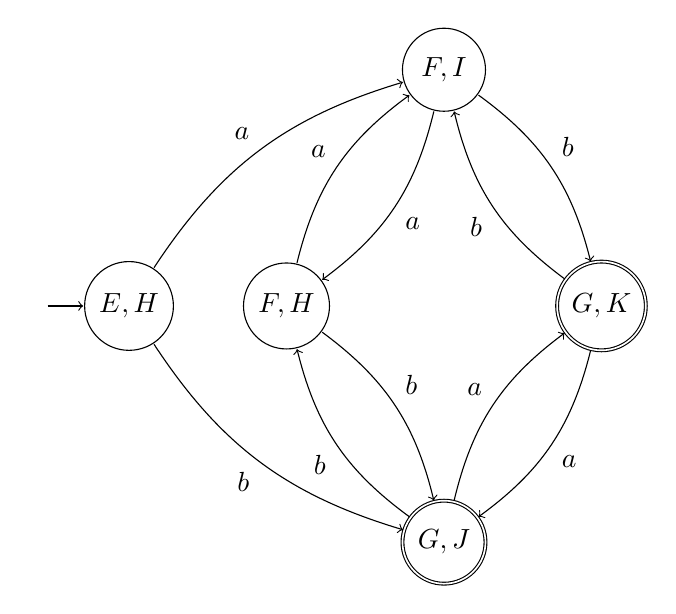
\begin{tikzpicture}[accepting=accepting by gdouble, initial text =, bend angle=20]
\tikzset{sommet/.style = {circle, draw, minimum size = 30 pt, >=latex}}                
\node[sommet, initial]   (EH) at  (0, 0) {$E, H$};
\node[sommet]            (FI) at  (4, 3) {$F, I$};
\node[sommet]            (FH) at  (2, 0) {$F, H$};
\node[sommet, accepting] (GJ) at  (4,-3) {$G, J$};
\node[sommet, accepting] (GK) at  (6, 0) {$G, K$};
\draw[->, bend left]  (EH) edge node[above left]  {$a$} (FI);
\draw[->, bend right] (EH) edge node[below left]  {$b$} (GJ);
\draw[->, bend left]  (FI) edge node[below right] {$a$} (FH);
\draw[->, bend left]  (FI) edge node[above right] {$b$} (GK);
\draw[->, bend left]  (FH) edge node[above left]  {$a$} (FI);
\draw[->, bend left]  (FH) edge node[above right] {$b$} (GJ);
\draw[->, bend left]  (GJ) edge node[above left]  {$a$} (GK);
\draw[->, bend left]  (GJ) edge node[below left]  {$b$} (FH);
\draw[->, bend left]  (GK) edge node[below left]  {$b$} (FI);
\draw[->, bend left]  (GK) edge node[below right] {$a$} (GJ);
\end{tikzpicture}
\end{center}
\end{Exercise}
%-------------------------------------------------------------------------------
\newpage
%-------------------------------------------------------------------------------
\begin{Exercise}
On numérote les sommets par $k_1 + n_1.k_2$ où $k-1$ et $k_2$ sont les indices respectivement du premier et du second automate et $n_1$ est la taille du premier.
\begin{lstlisting}
let produit q1 q2 =
  let (n1, delta1, f1) = q1 in
  let (n2, delta2, f2) = q2 in
  let n = n1*n2 in
  let delta = Array.make n (0,0) in
  let f = Array.make n false in
  for k1 = 0 to (n1 - 1) do
    for k2 = 0 to (n2 - 1) do
      let k = k1 + k2*n1 in
      let (a1, b1) = delta1.(k1) in
      let (a2, b2) = delta2.(k2) in
      delta.(k) <- (a1 + a2*n1, b1 + b2*n1);
      f.(k) <- f1.(k1) && f2.(k2) done done;
  (n, delta, f);;
\end{lstlisting}
\end{Exercise}
%-------------------------------------------------------------------------------
%-------------------------------------------------------------------------------
\begin{Exercise}
De la même manière qu'à la question {\bf \ref{ques:delta}} on prouve, par récurrence su $|u|$ que
\[\delta_{{\cal A}\times {\cal A}'}^*\bigl((s, s'), u\bigr) = \bigl(\delta_{\cal A}^*(s, u), \delta_{{\cal A}'}^*(s', u)\bigr)\]

Si $(s, s')$ est accessible, on peut écrire $(s, s') = \delta_{{\cal A}\times {\cal A}'}^*\bigl((i_{\cal A}, i_{{\cal A}'}), u\bigr) = \bigl(\delta_{\cal A}^*(i_{\cal A}, u), \delta_{{\cal A}'}^*(i_{\cal A}, u)\bigr)$.

$u$ est reconnu par ${\cal A}$ si et seulement si il est reconnu par ${\cal A}'$ d'où $q\in F_{\cal A} \iff q'\in F_{{\cal A} '}$.
\end{Exercise}
%-------------------------------------------------------------------------------
%-------------------------------------------------------------------------------
\begin{Exercise}[label=ques:prod]
On considère  la projection de ${\cal A}\times{\cal A}'$ sur ${\cal A}$ : $(s, s') \mapsto s$ et on note $\varphi_1$ sa  restriction  à l'ensemble des états accessibles de ${\cal A}\times{\cal A}'$.

\begin{enumerate}
  \item Tout état $s$ de ${\cal A}$ est accessible donc il existe $u$ tel que $s = \delta_{\cal A}^*(i_{\cal A}, u)$. Si on note $s' = \delta_{{\cal A}'}^*(i_{\cal A}, u)$, on a $(s, s')$ accessible dans ${\cal A}\times{\cal A}'$ donc $s = \varphi_1(s, s')$. $\varphi_1$ est surjective.
  \item $\varphi_1(i_{{\cal A}\times {\cal A}'}) = \varphi_1(i_{{\cal A}},i_{{\cal A}'})=i_{{\cal A}}$.
  \item $\varphi_1\bigl(\delta_{{\cal A}\times {\cal A}'}(('s, s'), x)\bigr) = \varphi_1\bigl(\delta_{\cal A}(s, x),\delta_{{\cal A}'}(s', x)\bigr)
  = \delta_{\cal A}(s, x)=\delta_{\cal A}\bigl(\varphi_1(s, s'), x \bigr)$.
  \item Si $(s, s') \in F_{{\cal A}\times {\cal A}'}= F_{\cal A}\times F_{{\cal A}'}$ alors $\varphi_1(s, s') = s \in F_{\cal A}$.
  
  Inversement, pour $s \in F_{\cal A}$, il existe $s'\in F_{{\cal A}'}$ tel que $(s, s')$ est accessible dans ${\cal A}\times{\cal A}'$. La question précédente montre que $s'$ est final dans ${\cal A}'$ d'où $(s, s')\in F_{{\cal A}\times {\cal A}'}$. Ainsi $\varphi_1(s, s') \in  F_{\cal A}$ implique $(s, s')\in F_{{\cal A}\times {\cal A}'}$.
    On en conclut l'équivalence.
\end{enumerate}
Les 4 propriétés prouve que $\varphi_1$ est un morphisme d'automates de la partie accessible de ${\cal A}\times{\cal A}'$ vers ${\cal A}$.
De même la restriction de la seconde projection est un morphisme d'automates de la partie accessible de ${\cal A}\times{\cal A}'$ vers ${\cal A}'$.
\end{Exercise}
%-------------------------------------------------------------------------------
%-------------------------------------------------------------------------------
\subsection{Diagramme d'automates}
%-------------------------------------------------------------------------------
%-------------------------------------------------------------------------------
\begin{Exercise}
On nomme {\bf chemin} de $p$ vers $q$ une suite d'états vérifiant les propriétés de la définition.

\begin{itemize}
  \item $(p)$ est un chemin de $p$ vers $p$ donc $p\equiv p$.
  \item Si $p\equiv q$ on considère un chemin $(p, s_1, \ldots, s_{k-1}, q)$ de $p$ vers $q$.
  
  $(q, s_{k-1}, \ldots, s_1, p)$ est alors un chemin de $q$ vers $p$ : $p\equiv q \Longrightarrow q\equiv p$.
  \item Si $p \equiv q$ et $q\equiv r$ on considère un chemin $(p, s_1, \ldots, s_{k-1}, q)$ de $p$ vers $q$ et un chemin $(q, t_1, \ldots, t_{l-1}, r)$ de $q$ vers $r$. 
  
  $(p, s_1, \ldots, s_{k-1}, q, t_1, \ldots, t_{l-1}, r)$ est alors un chemin de $p$ vers $r$ : $p\equiv q \wedge q \equiv r \Longrightarrow q\equiv r$.
\end{itemize}
$\equiv$ est une relation d'équivalence.
\end{Exercise}
%-------------------------------------------------------------------------------
%-------------------------------------------------------------------------------
\begin{Exercise}[label=ques:stable]
On considère un chemin $(s_0, s_1, \ldots, s_{k-1}, s_k)$ avec $s_0=p$ et $s_k=q$ pour $p\equiv q$.

Si on a $\varphi(s_i) = \varphi(s_{i+1})$ alors $\varphi\bigl(\delta_{\cal B}(s_i, x)\bigr) = \delta_{\cal A}\bigl(\varphi(s_i), x)\bigr)
= \delta_{\cal A}\bigl(\varphi(s_{i+1}), x)\bigr) = \varphi\bigl(\delta_{\cal B}(s_{i+1}, x)\bigr)$.

De même pour $\psi$.

Ainsi, si on note $t_i = \delta_{\cal B}(s_i, x)$, on a toujours $\varphi(t_i) = \varphi(t_{i+1})$ ou  $\psi(t_i) = \psi(t_{i+1})$ donc

$(t_0, t_1, \ldots, t_{k-1}, t_k)$ est un chemin de $\delta_{\cal B}(p, x)$ vers $\delta_{\cal B}(q, x)$.
$p\equiv q \Longrightarrow \delta_{\cal B}(p, x)\equiv \delta_{\cal B}(q, x)$.
\end{Exercise}
%-------------------------------------------------------------------------------
%-------------------------------------------------------------------------------
\begin{Exercise}[label=ques:final]
On suppose $p\equiv q$ et on considère un chemin $(s_0, s_1, \ldots, s_{k-1}, s_k)$ avec $s_0=p$ et $s_k=q$.

Montrons que $s_i\in F_{\cal B} \Longrightarrow s_{i+1} \in F_{\cal B}$ pour $i< k$.
\begin{itemize}
  \item Si on a $\varphi(s_i) = \varphi(s_{i+1})$, on sait que $s_i\in F_{\cal B}$ donc $\varphi(s_i)\in F_{\cal A}$ d'où $\varphi(s_{i+1})\in F_{\cal A}$ 
  
  puis $s_{i+1} \in F_{\cal B}$ d'après la propriété $(3)$ d'un morphisme.
  \item De même si on a $\psi(s_i) = \psi(s_{i+1})$.
\end{itemize}

On en déduit que si $s_0 = p\in F_{\cal B}$ alors $s_i\in F_{\cal B}$ pour tout $i$ donc $q = s_k\in F_{\cal B}$.

De même, par symétrie de $\equiv$, $p\equiv q$ et $q$ final impliquent $p$ final.
\end{Exercise}
%-------------------------------------------------------------------------------
%-------------------------------------------------------------------------------
\begin{Exercise}[label=ques:coprod1]

\begin{itemize}
\item L'ensemble des sommets est ${\cal C} = \{S_0, S_1, \ldots, S_{\ell - 1}\}$.

\item L'exercice {\bf\ref{ques:stable}} montre que si on a $[s] = [t]$ alors $[\delta_{\cal B}(s, x)] = [\delta_{\cal B}(t, x)]$. 

On peut donc définir $\delta_{\cal C}([s], x) =[\delta_{\cal B}(s, x)]$. 

\item L'exercice {\bf\ref{ques:final}} montre que, pour $[s] = [t]$, $s\in F_{\cal B}\Longrightarrow t\in F_{\cal B}$. La propriété $s\in F_{\cal B}$ ne dépend donc pas du représentant de $[s]$ et on peut définir sans ambiguïté $F_{\cal C}$ comme l'ensemble des classes d'équivalence des éléments de $F_{\cal B}$.
\end{itemize}
Ainsi $\langle {\cal C}, [i_{\cal B}], \delta_{\cal C}, F_{\cal C}\rangle$ est un automate.

\begin{enumerate}
\item Par construction $\eta$ : $s \mapsto [\eta]$ est surjective.
\item $\eta(i_{cal B}) = [i_{\cal B}] = i_{\cal C}$.
\item $\eta\bigl(\delta_{\cal B}(s, x)\bigr) = [\delta_{\cal B}(s, x)] = \delta_{\cal C}([s], x)=\delta_{\cal C}\bigl(\eta(s), x\bigr)$.
\item On a vu que $\eta(s) = [s] \in F_{\cal C}$ équivaut à $s \in  F_{\cal B}$. 
\end{enumerate}

Ainsi $\eta$ est un morphisme d'automates de ${\cal B}$ vers ${\cal C}$.
\end{Exercise}
%-------------------------------------------------------------------------------
%-------------------------------------------------------------------------------
\begin{Exercise}[label=ques:coprod2]
On veut $\eta = \varphi' \circ \varphi$, donc on doit définir $\varphi'(t) = [s]$ pour $t=\varphi(s)$.

Il reste à prouver que $\varphi'$ est bien défini. Or $t = \varphi(s) = \varphi(s')$ implique que $s\equiv s'$ donc $[s] = [s']$ : la définition de $\varphi'(t)$ ne dépend pas de l’antécédent choisi. De plus $\varphi$ est surjective donc on peut définir $\varphi'(t)$ pour tout état $t\in {\cal A}$.

\medskip

Pour $t\in {\cal A}$ on considère $s\in {\cal B}$ tel que $t=\varphi(s)$ dans les deux derniers items.

On a alors $\varphi'(t) = \varphi'\circ \varphi(s) = \eta(s)$.

\begin{enumerate}
\item Pour tout état $[s]$ de ${\cal C}$, $[s] = \varphi'(t)$ avec $t=\varphi(s)$ : $\varphi'$ est surjective.
\item $i_{\cal A} = \varphi(i_{\cal B})$ donc $\varphi'(i_{\cal A}) = [i_{\cal B}] = i_{\cal C}$.
\item $\varphi'\bigl(\delta_{\cal A}(t, x)\bigr) = \varphi'\bigl(\delta_{\cal A}(\varphi(s), x)\bigr)
=\varphi'\circ \varphi \bigl(\delta_{\cal A}(s, x)\bigr)
=\eta\bigl(\delta_{\cal A}(s, x)\bigr)
=\delta_{\cal C}\bigl(\eta(s), x\bigr)
= \delta_{\cal C}\bigl(\varphi'(t), x\bigr)$.
\item $t = \varphi(s)\in F_{\cal A} \iff s \in F_{\cal B} \iff \eta(s) \in F_{\cal C}  \iff \varphi'(t) \in F_{\cal C}$.
\end{enumerate}
$\varphi'$ est un morphisme d'automates de ${\cal A}$ vers ${\cal C}$.

\medskip

De même on définit un morphisme d'automates de ${\cal A}'$ vers ${\cal C}$ par $\psi'(t) = [s]$ pour $t = \psi(s)$.
\end{Exercise}
%-------------------------------------------------------------------------------
\newpage
%-------------------------------------------------------------------------------
\begin{Exercise}
Pour obtenir une complexité linéaire relativement à la taille de l'automate on va maintenir un tableau de substitution des valeurs. Quand on lit une valeur
\begin{itemize}
  \item soit elle a déjà été rencontrée et sa valeur de substitution est connue, on l'applique
  \item soit elle est nouvelle, on définit sa substitution en incrémentant un compteur et on l'applique.
\end{itemize}
On doit faire une première lecture du tableau pour déterminer la valeur maximale. On suppose le tableau non vide.
\begin{lstlisting}
let maxi_tableau t =
  let n = Array.length t in
  let maxi = ref t.(0) in
  for i = 1 to (n-1) do
    if t.(i) > !maxi then maxi := t.(i) done;
  !maxi;;
\end{lstlisting}

\begin{lstlisting}
let renomme t =
  let n = Array.length t in
  let maxi = maxi_tableau t in
  let code = Array.make (maxi + 1) None in
  let out = Array.make n (-1) in
  let subs = ref 0 in
  for i = 0 to (n-1) do
    let k = t.(i) in
    match code.(k) with
    |None -> code.(k) <- Some !subs;
             out.(i) <- !subs;
             incr subs
    |p -> out.(i) <- p done;
  out;;
\end{lstlisting}

La complexité est en ${\cal O}(n +l)$ où $l$ est le maximum du tableau. Dans le cas du sujet, $l$ est majoré par $n$ d'où la complexité linéaire.
\end{Exercise}
%-------------------------------------------------------------------------------
%-------------------------------------------------------------------------------
\begin{Exercise}
La structure naturelle pour gérer une relation d'équivalence  est la structure {\bf union-find} telle qu'utilisée dans l'algorithme de Kruskal.
\begin{lstlisting}
let creerUF n = 
  Array.init n (fun i -> i);; 
  
let rec find u i = 
  if u.(i) <> i 
  then find u (u.(i)) 
  else i;;
  
let union u i j = 
  let k = find u i in 
  let l = find u j in 
  if k <> l then u.(k) <- l;;
\end{lstlisting}

On peut utiliser la compression dans \type{find} :
\begin{lstlisting}
let rec find u i = 
  if u.(i) <> i then u.(i) <- find u (u.(i));
  u.(i);;
\end{lstlisting}

\newpage

On crée donc les classes d'équivalences par adjonction des classes des paires d'éléments qui ont une image en commun. Il faudra ensuite remplacer, dans le tableau, les antécédents par la racine des arbres.

\begin{lstlisting}
let relation phi psi =
  let n = Array.length phi in
  let uf = creerUF n in
  for i = 0 to (n - 2) do
    for j = (i + 1) to (n - 1) do
      if phi.(i) = phi.(j) || psi.(i) = psi.(j) 
      then union uf i j done done;
  for k = 0 to (n-1) do uf.(k) <- find uf k done;
  renomme uf;;
\end{lstlisting}

\end{Exercise}
%-------------------------------------------------------------------------------
%-------------------------------------------------------------------------------
%-------------------------------------------------------------------------------
\section{Réductions d'automates}
%-------------------------------------------------------------------------------
%-------------------------------------------------------------------------------
%-------------------------------------------------------------------------------
\subsection{Existence et unicité}
%-------------------------------------------------------------------------------
%-------------------------------------------------------------------------------
\begin{Exercise}[label=ques:coprod3]
On définit ${\cal B}$ comme la partie accessible de ${\cal A}\times {\cal A}'$, la question {\bf \ref{ques:prod}} montre qu'il existe des morphismes $\varphi$ et $\psi$ respectivement de  ${\cal B}$ vers  ${\cal A}$ et de  ${\cal B}$ vers ${\cal A}'$.

Les questions {\bf \ref{ques:coprod1}} et {\bf \ref{ques:coprod2}} permettent alors de définir un automate ${\cal C}$ et deux morphismes $\varphi'$ et $\psi'$ respectivement de  ${\cal A}$ vers  ${\cal C}$ et de  ${\cal A}'$ vers ${\cal C}$.

\end{Exercise}
%-------------------------------------------------------------------------------
%-------------------------------------------------------------------------------
\begin{Exercise}
Dans la partie accessible de ${\cal A}_3\times {\cal A}_4$, on a $(E, H) \equiv (F, H) \equiv (F, I)$ et $(G, J) \equiv (G,K)$.

0 représente la classe de $(E, H)$, c'est l'état initial, 1 est la classe de $(G, J)$, c'est le seul état final.

L'automate ${\cal C}$ est isomorphe à l'automate ${\cal A}_2$.

On a alors $\varphi'(E) = \varphi'(F) =0$, $\varphi'(H) = 1$, $\psi'(H)=\psi'(I)=0$ et $\psi'(J)=\psi'(K) = 1$.

\end{Exercise}
%-------------------------------------------------------------------------------
%-------------------------------------------------------------------------------
\begin{Exercise}
${\cal A}$ et ${\cal A}'$ sont deux automates reconnaissant le même langage $L$ et de cardinal minimal dans ${\frak K}_L$.

Dans la construction de la question {\bf \ref{ques:coprod3}} on définit un automate $\cal C$ et deux morphismes $\varphi'$ et $\psi'$ respectivement de  ${\cal A}$ vers  ${\cal C}$ et de  ${\cal A}'$ vers ${\cal C}$.

D'après la question {\bf \ref{ques:delta}}, ${\cal C}$ reconnaît aussi $L$. Son cardinal est donc supérieur ou égal à celui de ${\cal A}$ et de ${\cal A}'$ ; comme $\varphi'$ et $\psi'$ sont surjectifs, le cardinal de ${\cal C}$ est inférieur ou égal à celui de ${\cal A}$ et de ${\cal A}'$. On en déduit que les 3 automates ont même cardinal.

D'après la question {\bf \ref{ques:isom}} on peut conclure que $\varphi'$ est un isomorphisme de ${\cal A}$ vers ${\cal C}$ et $\psi'$ un isomorphisme de ${\cal A}'$ vers ${\cal C}$ donc $\psi'^{-1}\circ \varphi$ est un isomorphisme de ${\cal A}$ vers ${\cal A}'$.
\end{Exercise}
%-------------------------------------------------------------------------------
%-------------------------------------------------------------------------------
\begin{Exercise}
C'est la même démonstration, sans supposer que ${\cal A}'$ est de cardinal minimal.

On prouve encore que $varphi'$ est un isomorphisme de ${\cal A}$ vers ${\cal C}$.

Dans ce cas $\varphi'^{-1}\circ \psi'$ est un morphisme de ${\cal A}'$ vers ${\cal A}$.

{\it Il aurait été judicieux d'inverser les deux questions.}
\end{Exercise}
%-------------------------------------------------------------------------------
\newpage
%-------------------------------------------------------------------------------
\subsection{Construction}
%-------------------------------------------------------------------------------
%-------------------------------------------------------------------------------
\begin{Exercise}
Pour fusionner l'automate en assimilant les états $O$ et $P$, il faut aussi fusionner les états $Q$ et $T$ pour que l'image de l'état $(O, P)$ par la transition $b$ puisse être définie. Le morphisme est représenté par les antécédents de chaque états de ${\cal A}_6^{O, P}$.
\begin{center}
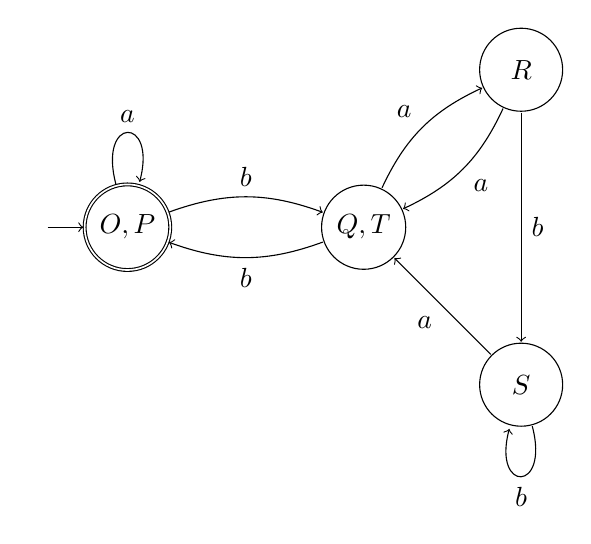
\begin{tikzpicture}[accepting=accepting by gdouble, initial text =, bend angle=20]
\tikzset{sommet/.style = {circle, draw, minimum size = 30 pt, >=latex}}                
\node[sommet, initial, accepting]   (OP) at  (0, 0) {$O, P$};
\node[sommet] (QT) at  (3, 0) {$Q, T$};
\node[sommet] (S)  at  (5,-2) {$S$};
\node[sommet] (R)  at  (5, 2) {$R$};
\draw[->] (OP) edge[loop above] node[above]       {$a$} (OP);
\draw[->]  (S) edge[loop below] node[below]       {$b$}  (S);
\draw[->, bend left]  (OP) edge node[above]       {$b$} (QT);
\draw[->, bend left]  (QT) edge node[below]       {$b$} (OP);
\draw[->, bend left]  (R)  edge node[below right] {$a$} (QT);
\draw[->, bend left]  (QT) edge node[above left]  {$a$}  (R);
\draw[->]             (S)  edge node[below left]  {$a$} (QT);
\draw[->]             (R)  edge node[right]       {$b$}  (S);
\end{tikzpicture}
\end{center}
\end{Exercise}
%-------------------------------------------------------------------------------
%-------------------------------------------------------------------------------
\begin{Exercise}
Il n'est pas possible de fusionner $Q$ et $R$ car les transitions avec la lettre $b$ donnent respectivement $O$ et $S$. Or $O$ est final alors que $S$ ne l'est pas, il ne sera donc pas possible de les fusionner en respectant la finalité des états dans un morphisme.
\end{Exercise}
%-------------------------------------------------------------------------------
%-------------------------------------------------------------------------------
\begin{Exercise}
On peut encore fusionner $R$ et $S$.
\begin{center}
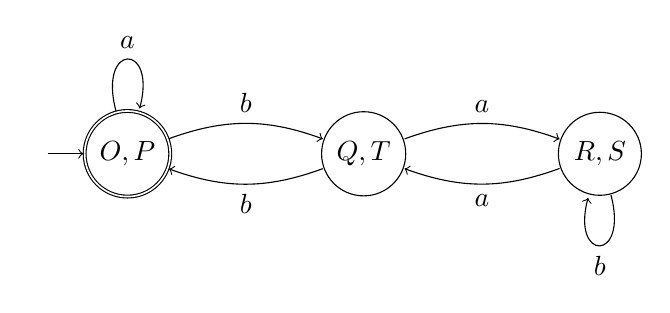
\begin{tikzpicture}[accepting=accepting by gdouble, initial text =, bend angle=20]
\tikzset{sommet/.style = {circle, draw, minimum size = 30 pt, >=latex}}                
\node[sommet, initial, accepting]   (OP) at  (0, 0) {$O, P$};
\node[sommet] (QT) at  (3, 0) {$Q, T$};
\node[sommet] (RS) at  (6, 0) {$R, S$};
\draw[->] (OP) edge[loop above] node[above]       {$a$} (OP);
\draw[->] (RS) edge[loop below] node[below]       {$b$} (RS);
\draw[->, bend left]  (OP) edge node[above]       {$b$} (QT);
\draw[->, bend left]  (QT) edge node[below]       {$b$} (OP);
\draw[->, bend left]  (QT) edge node[above]       {$a$} (RS);
\draw[->, bend left]  (RS) edge node[below]       {$a$} (QT);
\end{tikzpicture}
\end{center}
\end{Exercise}
%-------------------------------------------------------------------------------
%-------------------------------------------------------------------------------
\begin{Exercise}
C'est encore un parcours de graphe, on part depuis tous les sommets de $F\times (Q\setminus F) \cup (Q\setminus F) \times F$.
\begin{lstlisting}
let table_de_predecesseurs q =
  let (n, delta, f) = q in
  let pred = Array.make_matrix n n false in
  let rec visiter p q =
    if not pred.(p).(q)
    then begin pred.(p).(q) <- true;
         let pa, pb = delta.(p) in
         let qa, qb = delta.(q) in
         visiter pa qa;
         visiter pb qb end in
  for p = 0 to (n-1) do
    for q = 0 to (n-1) do
      if f.(p) <> f.(q) then visiter p q done done;
  pred;;
\end{lstlisting}
On ne traite chaque paire de sommets qu'au plus une fois et on fait alors deux appels récursifs : la complexité est en ${\cal O}(n^2)$.

\medskip

Il y a probablement une erreur dans l'énoncé : les paires d'états accessibles depuis une paire de points contenant un seul point final ne sont pas vraiment intéressants. On veut plutôt les paires qui parviennent à une paire final-non final.

On modifie donc le sujet avec les arcs allant d'un sommet $\bigl(\delta(p, x), \delta(q,x)\bigr)$ vers $(p, q)$.

On a maintenant une structure qui n'est plus celle d'un automate déterministe (c'est un automate déterministe) d'où la nécessite de parler de graphe.

On commence par créer le graphe avec une matrice des listes d'adjacence.

\begin{lstlisting}
let graphe q = 
  let n, delta, f = q in
  let adj = Array.make_matrix n n [] in
  for p = 0 to (n-1) do
    for q = 0 to (n-1) do
      let pa, pb = delta.(p) in
      let qa, qb = delta.(q) in
      adj.(pa).(qa) <- (p, q) :: adj.(pa).(qa);
      adj.(pb).(qb) <- (p, q) :: adj.(pb).(qb) done done;
  adj;;
\end{lstlisting}
 On reprend alors le parcours avec le tableau.
\begin{lstlisting}
let table_de_predecesseurs q =
  let (n, delta, f) = q in
  let g = graphe q in
  let pred = Array.make_matrix n n false in
  let rec visiter (p, q) =
    if not pred.(p).(q)
    then begin pred.(p).(q) <- true;
         List.iter visiter g.(p).(q) end in
  for p = 0 to (n-1) do
    for q = 0 to (n-1) do
      if f.(p) <> f.(q) then visiter (p, q) done done;
  pred;;
\end{lstlisting}
\end{Exercise}
%-------------------------------------------------------------------------------
%-------------------------------------------------------------------------------
\begin{Exercise}
{\bf On utilise la fonction de calculs des prédécesseurs modifiée.}

Si deux états $p$ et $q$ d'un automate ${\cal A}$ sont marqués à \type{false} dans le tableau des prédécesseurs, cela signifie que, pour tout mot $u$, $\delta^*(p, u)$ et $\delta^*(q, u)$ sont finaux en même temps. On note $\equiv_F$ cette relation, il est facile de montrer que c'est une relation d'équivalence.

Si on a $p\equiv_Fq$ alors on doit avoir $\delta(p, x) \equiv_F \delta(q, x)$ car sinon un mot $u$ enverrait $\delta(p, x)$ dans $F$ et $\delta(q, x)$ dans $Q\setminus F$ (ou l'inverse et le mot $xu$ aurait la même propriété pour $p$ et $q$ ce qui est exclu.

L'action du mot vide montre que, si $p\equiv_F q$ alors $p$ et $q$ sont dans $F$ en même temps.

\medskip

On peut ainsi définir un automate ${\cal A}_0$ à partir des classes d'équivalence, comme à la question {\bf \ref{ques:coprod1}},  ainsi qu'un morphisme de ${\cal A}$ vers ${\cal A}_0$. On a vu que ${\cal A}_0$ reconnaît le même langage que ${\cal A}$.

Dans ${\cal A}_0$, deux états distincts peuvent être séparés par un mot : pour $[p] \ne [q]$ on a $(p, q)$ marqué comme \type{true} dans la table des prédécesseurs donc il existe $u$ tel que il existe $u$ tel que $\delta^*(p, u)\in F$ et $\delta^*(q, u)\not \in F$ (ou l'inverse). S'il existe un morphisme $\psi'$ de ${\cal A}_0$ vers ${\cal A}'$ alors on ne peut avoir $\psi'([p]) = \psi'([q])$ car le transporté par $u$ devrait être à la fois final et non final en raison des propriétés d'un morphisme.

En particulier le morphisme de ${\cal A}_0$ vers un automate minimal est injectif donc c'est un isomorphisme ; on en déduit que ${\cal A}_0$ est minimal.

\newpage

On commence par la définition des classes d'équivalences. La fonction renvoie deux tableaux :
\begin{itemize}
  \item un tableau donnant le numéro de classe pour chaque état 
  \item et tableau donnant un représentant de chaque classe.
\end{itemize}
\begin{lstlisting}
let equivalence q = 
  let n, delta, f = q in
  let pred = table_de_predecesseurs q in
  let classe = Array.make n (-1) in
  let compteur = ref 0 in
  for p = 0 to (n-1) do
    if classe.(p) = -1
    then begin classe.(p) <- !compteur;
         for q = (p+1) to (n-1) do
           if not pred.(p).(q) 
           then classe.(q) <- !compteur done;
         incr compteur end 
    done;
  let repr = Array.make !compteur (-1) in
  for p = 0 to (n-1) do repr.(classe.(p)) <- p done; 
  classe, repr;;        
\end{lstlisting}

\begin{lstlisting}
let reduit q = 
  let n, delta, f = q in
  let classe, repr = equivalence q in
  let p = Array.length repr in
  let delta1 = Array.make p (0,0) in
  let f1 = Array.make p false in
  for i = 0 to (p-1) do
    let sa, sb = delta.(repr.(i)) in
    delta1.(i) <- (classe.(sa), classe.(sb));
    f1.(i) <- f.(repr.(i)) done;
  (p, delta1, f1);;
\end{lstlisting}
\end{Exercise}
%-------------------------------------------------------------------------------
%-------------------------------------------------------------------------------
%-------------------------------------------------------------------------------
\end{document}
%-------------------------------------------------------------------------------
%-------------------------------------------------------------------------------
%-------------------------------------------------------------------------------




